\documentclass[aspectratio=169]{beamer}

% Theme and appearance
\usetheme{Madrid}
\usecolortheme{default}

% Packages
\usepackage[utf8]{inputenc}
\usepackage[T1]{fontenc}
\usepackage{amsmath}
\usepackage{amsfonts}
\usepackage{amssymb}
\usepackage{graphicx}
\usepackage{booktabs}
\usepackage{tikz}
\usepackage{pgfplots}
\pgfplotsset{compat=1.18}
\usepackage{algorithm}
\usepackage{algorithmic}
\usepackage{hyperref}
\usepackage{subcaption}
\usepackage{multirow}
\usepackage{adjustbox}

% TikZ libraries
\usetikzlibrary{shapes,arrows,positioning,calc}

% Colors
\definecolor{berkeleyblue}{RGB}{0,50,98}
\definecolor{berkeleygold}{RGB}{253,181,21}
\definecolor{accent}{RGB}{255,107,107}

% Custom colors for the presentation
\setbeamercolor{structure}{fg=berkeleyblue}
\setbeamercolor{frametitle}{bg=berkeleyblue,fg=white}
\setbeamercolor{title}{fg=berkeleyblue}

% Presentation information
\title[Legal NLP Explainability]{Explainable AI for Legal Document Analysis: \\
A Multi-Method Approach to Clause Extraction}

\subtitle{W266 Final Project Presentation}

\author[Gabriel]{Perry Gabriel}

\institute[UC Berkeley]{
  School of Information \\
  University of California, Berkeley
}

\date{\today}

% Custom commands
\newcommand{\highlight}[1]{\textcolor{accent}{\textbf{#1}}}
\newcommand{\figpath}{../../visualizations/figures}

\begin{document}

% Title slide
\frame{\titlepage}

% Outline slide
\begin{frame}{Outline}
\tableofcontents
\end{frame}

% Include only introduction for testing
% Introduction Section

\section{Introduction}

\begin{frame}{Problem Statement}
\begin{itemize}
    \item \highlight{Legal document analysis} is crucial for contract review and compliance
    \item Traditional manual review is \highlight{time-consuming and error-prone}
    \item NLP models provide automation but lack \highlight{interpretability}
    \item Legal professionals need to understand \highlight{why} AI makes decisions
\end{itemize}

\vspace{0.5cm}
\begin{alertblock}{Research Question}
How can we develop explainable AI methods for automated legal clause extraction that provide interpretable insights for legal professionals?
\end{alertblock}
\end{frame}

\begin{frame}{Motivation}
\begin{columns}
\begin{column}{0.6\textwidth}
\textbf{Why Explainable AI in Legal Domain?}
\begin{itemize}
    \item \highlight{Regulatory compliance} requirements
    \item \highlight{Trust and transparency} for legal professionals
    \item \highlight{Error detection} and model debugging
    \item \highlight{Knowledge discovery} from legal patterns
\end{itemize}
\end{column}
\begin{column}{0.4\textwidth}
\begin{center}
% Show system architecture instead of placeholder
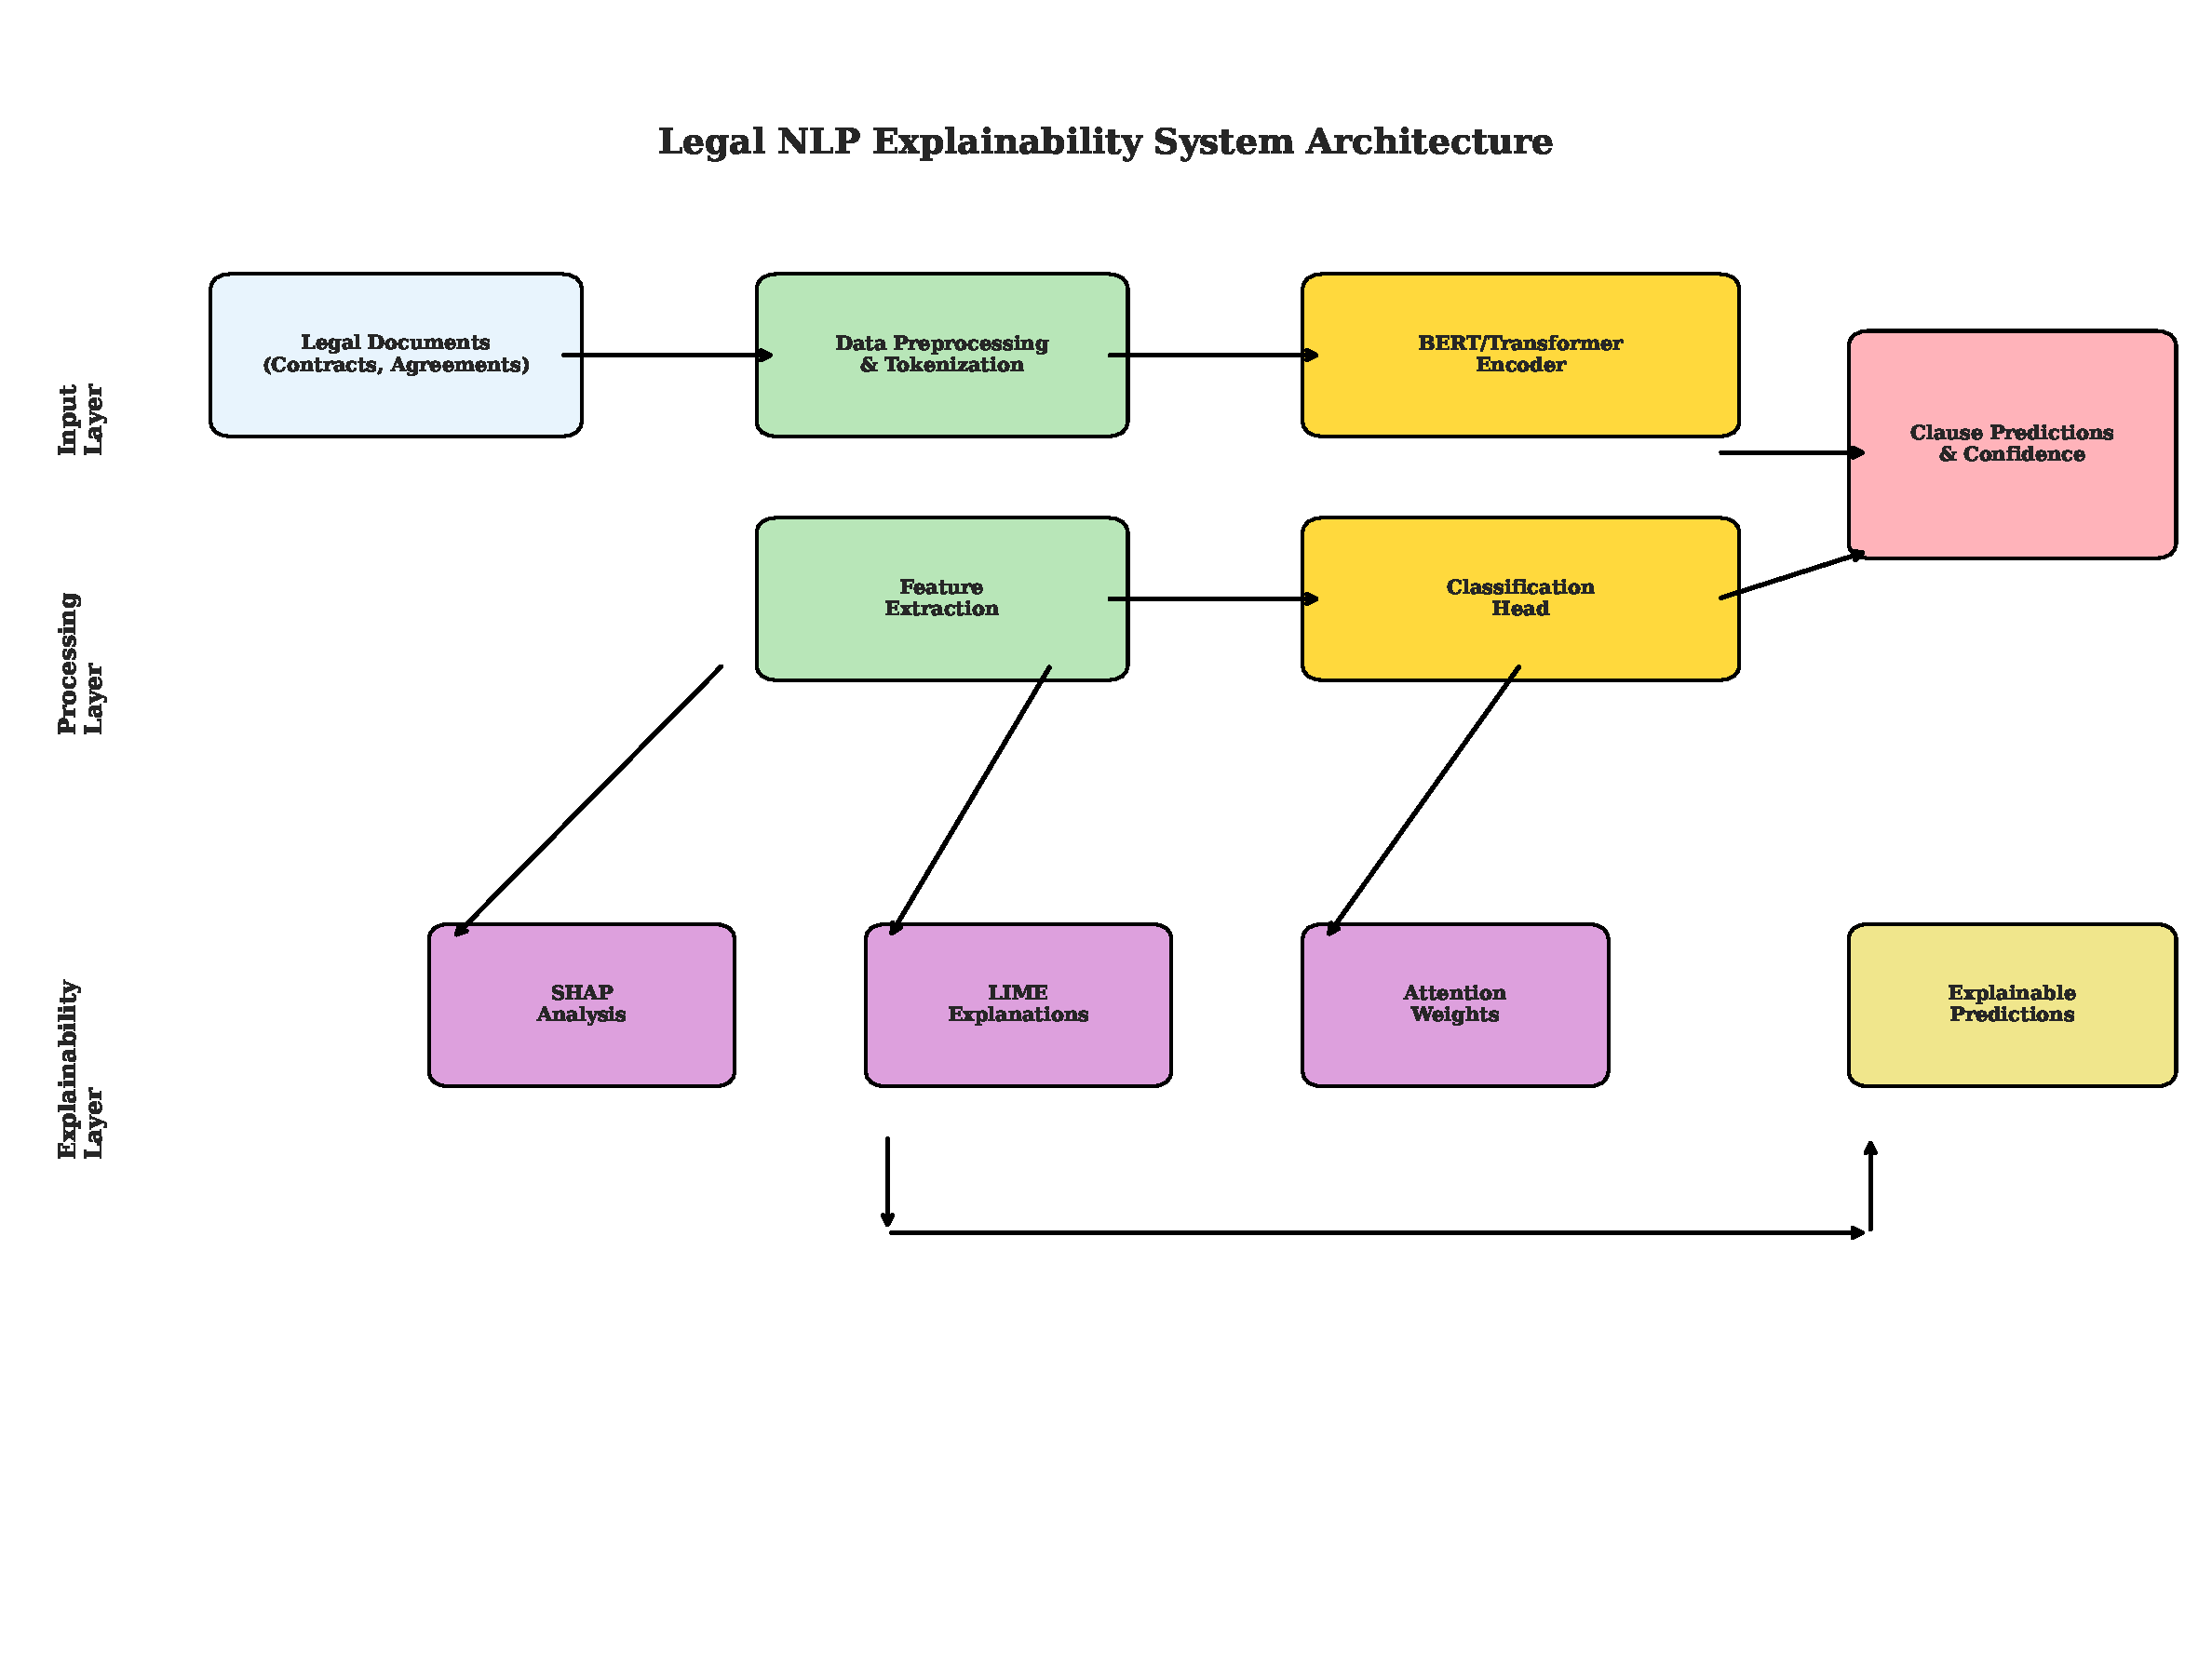
\includegraphics[width=\textwidth]{\figpath/system_architecture.pdf}
\end{center}
\end{column}
\end{columns}
\end{frame}

\begin{frame}{Project Scope}
\textbf{Objectives:}
\begin{enumerate}
    \item Develop a \highlight{BERT-based model} for clause extraction
    \item Implement \highlight{multiple explainability methods} (SHAP, LIME, Attention)
    \item Compare and evaluate \highlight{explanation quality}
    \item Create \highlight{interpretable visualizations} for legal professionals
\end{enumerate}

\vspace{0.5cm}
\textbf{Target Clauses:}
\begin{itemize}
    \item Termination clauses
    \item Limitation of liability
    \item Governing law
    \item Confidentiality provisions
    \item Payment terms
\end{itemize}
\end{frame}


% Thank you slide
\begin{frame}[plain]
\centering
\Huge \textcolor{berkeleyblue}{Thank You}
\vspace{1cm}

\Large Questions \& Discussion
\vspace{1cm}

\normalsize
\textbf{Contact:} pgabriel@berkeley.edu \\
\textbf{Repository:} \url{https://github.com/prgabriel/w266-project-legal-nlp-xai}
\end{frame}

\end{document}
